\label{subsub:expPreprocBenchmarks}

\ref{fig:wallClockDepthPreproc} shows the general runtime for party $P_0$.
Since all parties start and end the execution at the same time, runtimes between the parties are nearly the same.
One notes big differences in runtime beginning at depth 15.
Especially the \textit{gmp\_mpz\_approaches} suffer large performance degradation beyond depth 15.
\textit{new\_input\_type}, too, deteriorates from depth 15.
Yet, it still is about $5.2x$ to $6.3x$ faster than \textit{gmp\_mpz\_class}.
Differences in performance before depth 15 are larger when seen in relation, yet it is an impractical difference and thus negligible.

Differences in runtime are also present for constant depth and varying number of generated triples.
\ref{fig:wallClockIncNumPreproc} compares all approaches and plots their wall-clock time.
One notes an almost linear behavior of \textit{gmp\_mpz\_class}, especially for 64 bit.
\textit{base} and \textit{new\_input\_type} have an almost constant wall-clock time starting at $0.04$ seconds at one RDPF-Triple up to $0.23$ seconds for $100$ RDPF-triples. 
This is about $400x$ faster than \textit{gmp\_mpz\_class} for 256 bits and $290x$ faster than \textit{gmp\_mpz\_class} for the same bit size.

Each party stores its generated RDPF-triples in a local file (\ref{par:preliminariesRDPFs}).
Its storage requirements for 50 RDPF-triples of increasing depth are shown in \ref{fig:storageReqDepthPreproc}.
\textit{base} and \textit{gmp\_mpz\_class} for 64 bit have almost similar storage requirements for depths smaller 15.
\textit{mpz\_class} is structured in \textit{limbs}.
Each limb holds 8 bytes.
When values exceed a single limb, more limbs are allocated.
\code{mpz\_class} allocates these limbs at runtime, keeping track of its capacity and current length.
Therefore, even for the same bit size, a single \textit{mpz\_class} requires about $1.5x$ more storage than \code{uint64\_t} as used in \textit{base}.
\textit{gmp\_mpz\_class}, consequently, requires more storage than \textit{base}.
Recall that \textit{new\_input\_type} requires up to four times more RDPF-triples than \textit{base} during the online phase.
Therefore, around four times the storage is required.
Note that due to the exponential growth of the RDPF-trees, storage requirements increase heavily, again starting from depth 15.

This exponential growth can also be observed in \ref{fig:aesOpsDepthPreproc}.
The graph shows the amount of local AES operations for increasing depth.
As each tree is generated by using AES as length doubling PRG (\ref{sub:BGIDPFConstruction}), one needs at least $2^n$ local AES operations to construct a tree of depth $n$.
One observes \textit{new\_input\_type} executing four times more local AES operations than \textit{base}.
This is due to \textit{new\_input\_type} generating four times the RDPF-triples of \textit{base}.
Also, the \textit{gmp\_mpz\_class} for 64 bit executes less local AES operations than its larger fellows.
There is a difference of around 2 million local AES operations between 64 and 256 bit for depth 20.
This, however, has little to no impact on the general runtime as local AES operations on \code{\_\_m128i} vectors have nearly no overhead.

The reason for the runtime differences is found when taking a closer look at the performance when varying the bandwidth (\ref{fig:wallClockDecreasingBandwidthPreproc}).
When varying the bandwidth \textit{new\_input\_type} shows the biggest drop in performance.
As seen in \ref{fig:storageReqDepthPreproc}, \textit{new\_input\_type} has the largest storage requirements.
Thus, messages become larger slowing down the communication when the bandwidth drops.
A similar effect is observed for \textit{gmp\_mpz\_class}, yet, due to smaller storage requirements and thus smaller messages, not as large as for \textit{new\_input\_type}.

Varying the latency, however, slows down \textit{gmp\_mpz\_class} but not \textit{new\_input\_type}.
Taking a closer look at the implementation explains this issue:
In \textit{base} and \textit{new\_input\_type} message are stored in a buffer.
As each message has a fixed size of 8 bites, one can store messages in a buffer of fixed size.
Once the buffer is filled, one sends it and empties the buffer.
The set buffer size directly impacts the number of sent messages.
\textit{gmp\_mpz\_class} has no such buffer as messages are of variable size.
Therefore, messages are sent directly.
Also, \textit{gmp\_mpz\_class} sends two messages where \textit{base} and \textit{new\_input\_type} require only a single message as both the size of the data and the data itself are sent separately.
This not only results in increased message overhead as shown in \ref{fig:numSentMessagesIncDepthPreproc} but also in a higher performance degradation as latency increases.
Recall that \textit{mpz\_class} values need to be serialized before sending and deserialized when received (\ref{subsub:gmpCommunication}).
This significantly slows down each communication operation.
When tested, each sending operation including serialization required $0.01$ seconds on average, receiving took $0.02$ seconds on average.
This heavily impacts performance compared with $0.0001$ seconds for sending and $0.0025$ seconds for receiving a \code{uint64\_t} message.

Finally, bit operations on \code{mpz\_class} values are less performant than on \code{uint64\_t} values.
Testing showed that especially on \code{mpz\_class} values containing multiple limbs, bit shifts and XOR operations are around $5$ times slower than similar operations on \code{uint64\_t}.
The code used for proving the performance difference is given in \ref{lst:xorMpzVs64t}.

To conclude, \textit{gmp\_mpz\_class} is less performant for all bit sizes, depths, and number of generated RDPF-triples when compared to \textit{base} and \textit{new\_input\_type}.
It executes more local bit operations, sending operations, and receive operations.
All of which are slower than its \code{uint64\_t} equivalent.
This effect becomes particularly noticeable for depths greater than 15.
For smaller depths, however, \textit{gmp\_mpz\_class} is equally performant and storage efficient.
Its performance is also better than \textit{new\_input\_type} when bandwidth is small.
This, however, is reversed when latency fluctuates while bandwidth remains constant.
Therefore, preprocessing in \textit{gmp\_mpz\_class} can be preferred for larger bit sizes when depth and latency is small compared to \textit{new\_input\_type}.

\begin{figure}
    \centering 
    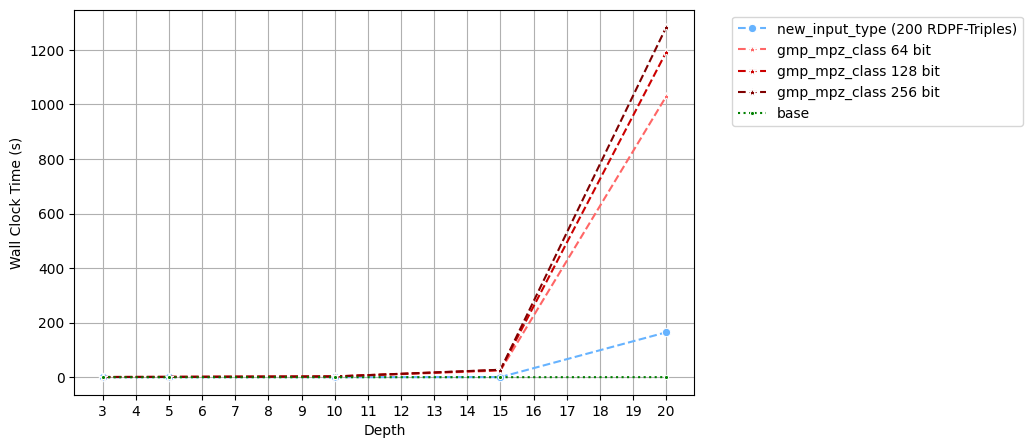
\includegraphics[width=0.8\textwidth]{plots/plots/preproc/wall_clock_preproc.png}
    \caption{Wall-Clock time for increasing depth and constant number of generated RDPF-Triples}
    \label{fig:wallClockDepthPreproc}
\end{figure}

\begin{figure}
    \centering
    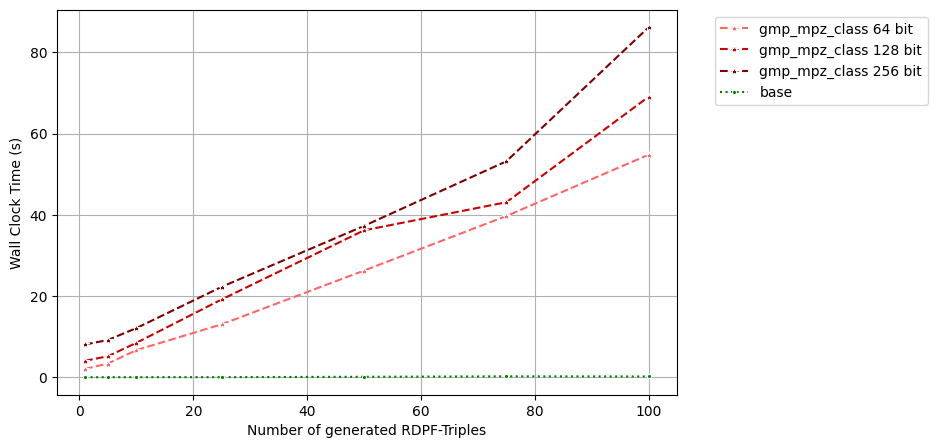
\includegraphics[width=0.8\textwidth]{plots/plots/preproc/wall_clock_incnum_preproc.png}
    \caption{Wall-Clock time for constant depth and increasing number of generated RDPF-Triples.
    Note here that \textit{new\_input\_type} is left out as it uses the same RDPF generation algorithm as \textit{base}.
    Therefore, both \textit{base} and \textit{new\_input\_type} have the exact same wall clock time for generating the same amount of RDPF-Triples of the same depth.
    }
    \label{fig:wallClockIncNumPreproc}
\end{figure}

\begin{figure}
    \centering
    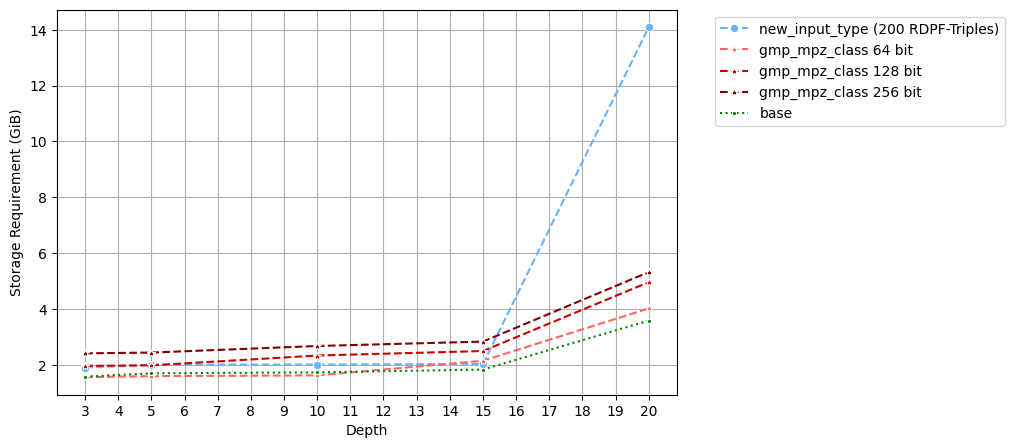
\includegraphics[width=0.8\textwidth]{plots/plots/preproc/storage_requirements_preproc.png}
    \caption{Storage Requirements for constant number of generated RDPF-Triples and increasing depth.}
    \label{fig:storageReqDepthPreproc}
\end{figure}

\begin{figure}
    \centering
    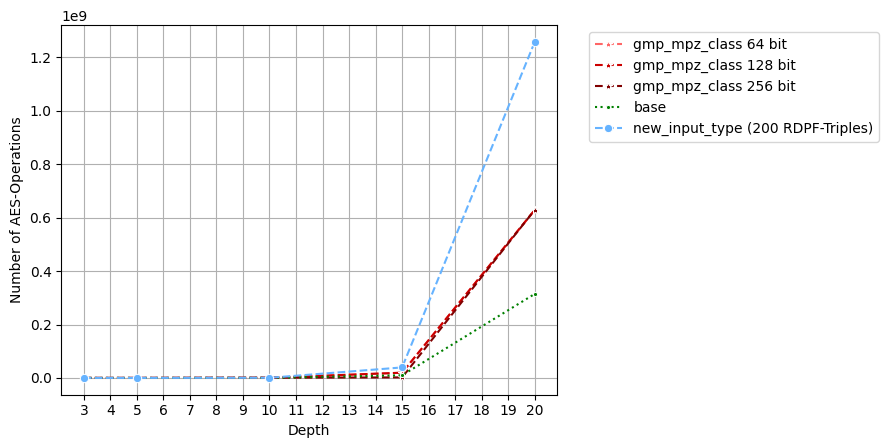
\includegraphics[width=0.8\textwidth]{plots/plots/preproc/aes_ops_preproc.png}
    \caption{Number of local AES operations for constant number of generated RDPF-Triples and increasing depth.}
    \label{fig:aesOpsDepthPreproc}
\end{figure}

\begin{figure}
    \centering
    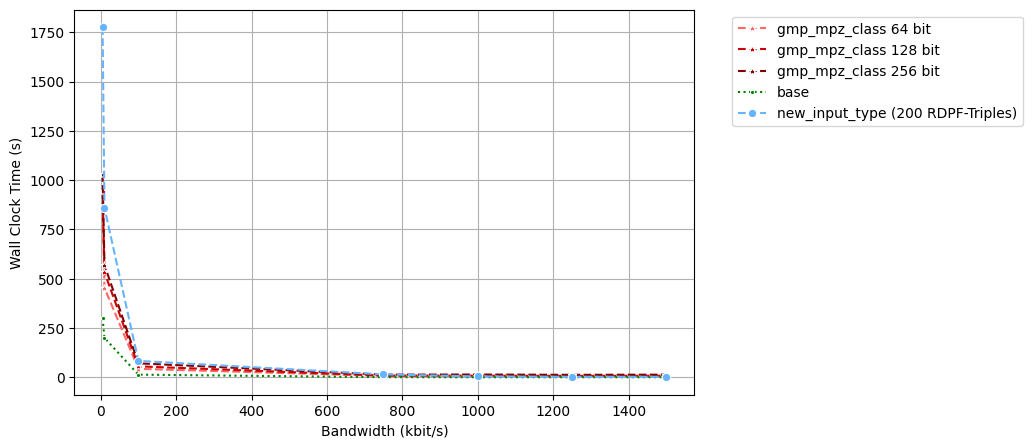
\includegraphics[width=0.8\textwidth]{plots/plots/preproc/time_decreasing_bandwidth_preproc.png}
    \caption{Wall-Clock time for increasing bandwidth, constant number of generated RDPF-Triples, constant depth, and constant latency.}
    \label{fig:wallClockDecreasingBandwidthPreproc}
\end{figure}

\begin{figure}
    \centering
    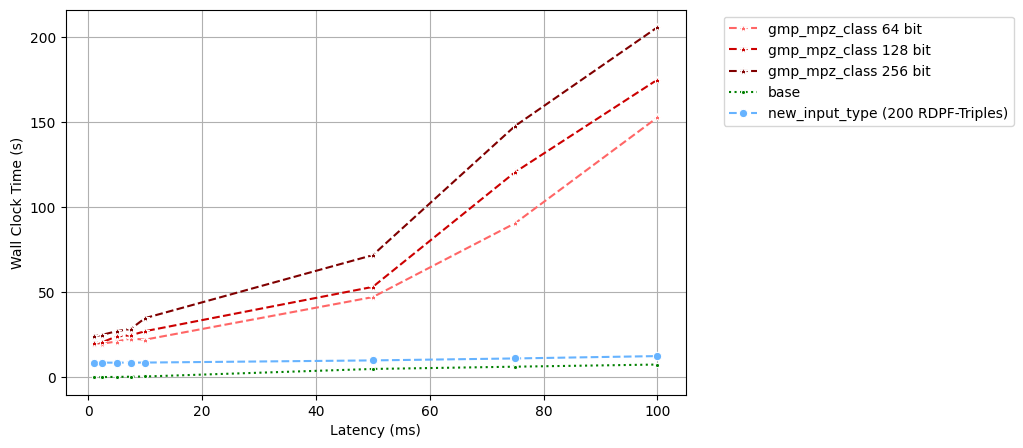
\includegraphics[width=0.8\textwidth]{plots/plots/preproc/time_decreasing_latency_preproc.png}
    \caption{Wall-Clock time for increasing latency, constant number of generated RDPF-Triples, constant depth, and constant bandwidth.}
    \label{fig:wallClockIncLatencyPreproc}
\end{figure}

\begin{figure}
    \centering
    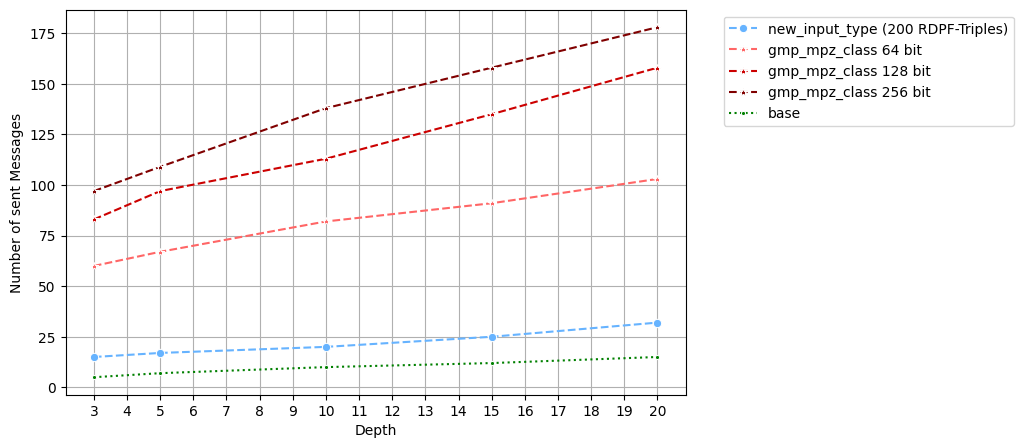
\includegraphics[width=0.8\textwidth]{plots/plots/preproc/sent_messages_preproc.png}
    \caption{Number of sent messages for constant number of generated RDPF-Triples and increasing depth.}
    \label{fig:numSentMessagesIncDepthPreproc}
\end{figure}